\section{Appendix A: R Code for Question 1}

To address the given task, we'll go through it step by step, writing R
code for each part. The task involves analyzing BMI data for Dutch boys
aged 10 to 11 years from the \texttt{dbbmi} dataset in the
\texttt{gamlss.data} package, fitting parametric distributions, and
selecting an appropriate one based on the analysis.

\hypertarget{instructions-on-how-to-analyse-the-first-data-set}{%
\subsection{Instructions on how to analyse the first data
set}\label{instructions-on-how-to-analyse-the-first-data-set}}

The first data set is a subset of Body Mass Index (BMI) data obtained
from the Fourth Dutch Growth Study, Fredriks et al.~2000 {[}1{]}. The
data contains BMI for different ages in years for Dutch boys. Each
student will be given a different age, for example, 10 to 11 years old.
The aim here is to find a suitable distribution of the BMI at this age.

\hypertarget{a-the-original-data-which-contains-all-ages-from-zero-to-twenty-two-exists-in-the-gamlss.data-package-under-the-name-of-dbbmi.-each-student-should-analyse-a-different-age.-here-we-give-an-example-how-to-analyse-age-10.-we-first-bring-the-data-set-in-r-and-then-create-a-subset-data.frame-containing-only-a-specific-age-here-from-10-11.-the-following-commands-can-be-used}{%
\subsubsection{(a) The original data, which contains all ages from zero
to twenty two, exists in the gamlss.data package under the name of
dbbmi. Each student should analyse a different age. Here we give an
example how to analyse age 10. We first bring the data set in R and then
create a subset data.frame containing only a specific age (here from
10-11). The following commands can be
used:}\label{a-the-original-data-which-contains-all-ages-from-zero-to-twenty-two-exists-in-the-gamlss.data-package-under-the-name-of-dbbmi.-each-student-should-analyse-a-different-age.-here-we-give-an-example-how-to-analyse-age-10.-we-first-bring-the-data-set-in-r-and-then-create-a-subset-data.frame-containing-only-a-specific-age-here-from-10-11.-the-following-commands-can-be-used}}

First, let's load the data, subset it for the specific age group, and
plot the histogram to find a suitable value for \texttt{nbins}.

\begin{Shaded}
\begin{Highlighting}[]
\CommentTok{\# suppress the warnings by setting warn={-}1 }
\FunctionTok{options}\NormalTok{(}\AttributeTok{warn=}\SpecialCharTok{{-}}\DecValTok{1}\NormalTok{) }

\CommentTok{\# Load the packages}
\FunctionTok{library}\NormalTok{(ggplot2)}
\FunctionTok{library}\NormalTok{(gamlss)}
\end{Highlighting}
\end{Shaded}

\begin{verbatim}
## Loading required package: splines
\end{verbatim}

\begin{verbatim}
## Loading required package: gamlss.data
\end{verbatim}

\begin{verbatim}
## 
## Attaching package: 'gamlss.data'
\end{verbatim}

\begin{verbatim}
## The following object is masked from 'package:datasets':
## 
##     sleep
\end{verbatim}

\begin{verbatim}
## Loading required package: gamlss.dist
\end{verbatim}

\begin{verbatim}
## Loading required package: nlme
\end{verbatim}

\begin{verbatim}
## Loading required package: parallel
\end{verbatim}

\begin{verbatim}
##  **********   GAMLSS Version 5.4-20  **********
\end{verbatim}

\begin{verbatim}
## For more on GAMLSS look at https://www.gamlss.com/
\end{verbatim}

\begin{verbatim}
## Type gamlssNews() to see new features/changes/bug fixes.
\end{verbatim}

\begin{Shaded}
\begin{Highlighting}[]
\FunctionTok{library}\NormalTok{(gamlss.ggplots)}
\end{Highlighting}
\end{Shaded}

\begin{verbatim}
## Loading required package: gamlss.foreach
\end{verbatim}

\begin{verbatim}
## Loading required package: foreach
\end{verbatim}

\begin{verbatim}
## Loading required package: doParallel
\end{verbatim}

\begin{verbatim}
## Loading required package: iterators
\end{verbatim}

\begin{Shaded}
\begin{Highlighting}[]
\FunctionTok{library}\NormalTok{(gamlss.add)}
\end{Highlighting}
\end{Shaded}

\begin{verbatim}
## Loading required package: mgcv
\end{verbatim}

\begin{verbatim}
## This is mgcv 1.9-0. For overview type 'help("mgcv-package")'.
\end{verbatim}

\begin{verbatim}
## Loading required package: nnet
\end{verbatim}

\begin{verbatim}
## 
## Attaching package: 'nnet'
\end{verbatim}

\begin{verbatim}
## The following object is masked from 'package:mgcv':
## 
##     multinom
\end{verbatim}

\begin{verbatim}
## Loading required package: rpart
\end{verbatim}

\begin{Shaded}
\begin{Highlighting}[]
\FunctionTok{library}\NormalTok{(gamlss.data)}
\FunctionTok{library}\NormalTok{(MASS)}

\CommentTok{\# Load the dataset}
\FunctionTok{data}\NormalTok{(dbbmi)}
\FunctionTok{summary}\NormalTok{(dbbmi)}
\end{Highlighting}
\end{Shaded}

\begin{verbatim}
##       age              bmi       
##  Min.   : 0.030   Min.   :11.17  
##  1st Qu.: 1.863   1st Qu.:15.96  
##  Median :10.450   Median :17.45  
##  Mean   : 9.291   Mean   :18.03  
##  3rd Qu.:15.130   3rd Qu.:19.60  
##  Max.   :21.700   Max.   :35.42
\end{verbatim}

\begin{Shaded}
\begin{Highlighting}[]
\CommentTok{\# Subset for ages 15 to 16}
\NormalTok{old }\OtherTok{\textless{}{-}} \DecValTok{15}
\NormalTok{dbbmi\_15 }\OtherTok{\textless{}{-}} \FunctionTok{with}\NormalTok{(dbbmi, }\FunctionTok{subset}\NormalTok{(dbbmi, age }\SpecialCharTok{\textgreater{}}\NormalTok{ old }\SpecialCharTok{\&}\NormalTok{ age }\SpecialCharTok{\textless{}}\NormalTok{ old }\SpecialCharTok{+} \DecValTok{1}\NormalTok{))}
\NormalTok{bmi15 }\OtherTok{\textless{}{-}}\NormalTok{ dbbmi\_15}\SpecialCharTok{$}\NormalTok{bmi}

\CommentTok{\# Plot the histogram; adjust nbins as needed to make the histogram look good}
\NormalTok{binwith }\OtherTok{=} \FloatTok{0.5}
\NormalTok{nbins }\OtherTok{=} \FunctionTok{trunc}\NormalTok{(}\FunctionTok{max}\NormalTok{(bmi15) }\SpecialCharTok{{-}} \FunctionTok{min}\NormalTok{(bmi15)) }\SpecialCharTok{/}\NormalTok{ binwith}

\FunctionTok{truehist}\NormalTok{(bmi15, }\AttributeTok{nbins=}\NormalTok{nbins)}
\end{Highlighting}
\end{Shaded}

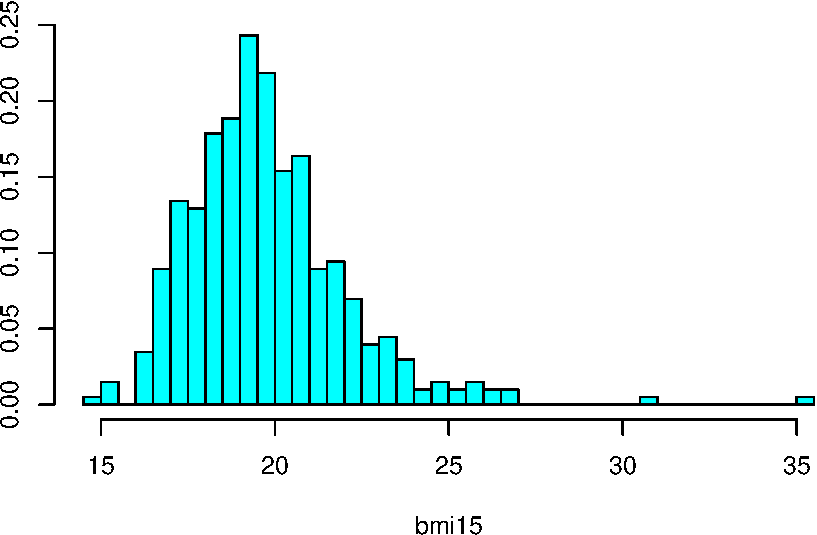
\includegraphics{assignment_q1_bmi_files/figure-latex/unnamed-chunk-1-1.pdf}

\begin{Shaded}
\begin{Highlighting}[]
\FunctionTok{density}\NormalTok{(bmi15, }\AttributeTok{cut =} \DecValTok{0}\NormalTok{)}
\end{Highlighting}
\end{Shaded}

\begin{verbatim}
## 
## Call:
##  density.default(x = bmi15, cut = 0)
## 
## Data: bmi15 (403 obs.);  Bandwidth 'bw' = 0.515
## 
##        x               y            
##  Min.   :14.70   Min.   :4.300e-07  
##  1st Qu.:19.78   1st Qu.:6.803e-04  
##  Median :24.87   Median :1.193e-02  
##  Mean   :24.87   Mean   :4.900e-02  
##  3rd Qu.:29.95   3rd Qu.:8.370e-02  
##  Max.   :35.03   Max.   :2.127e-01
\end{verbatim}

\begin{Shaded}
\begin{Highlighting}[]
\NormalTok{gamlss.ggplots}\SpecialCharTok{:::}\FunctionTok{y\_hist}\NormalTok{(dbbmi\_15}\SpecialCharTok{$}\NormalTok{bmi,}
                        \AttributeTok{from=}\FunctionTok{floor}\NormalTok{(}\FunctionTok{min}\NormalTok{(bmi15)), }
                        \AttributeTok{to=}\FunctionTok{ceiling}\NormalTok{(}\FunctionTok{max}\NormalTok{(bmi15)), }
                        \AttributeTok{binwidth=}\NormalTok{binwith,}
                        \AttributeTok{title=}\StringTok{"Histogram of BMI for 15 year olds"}\NormalTok{)}
\end{Highlighting}
\end{Shaded}

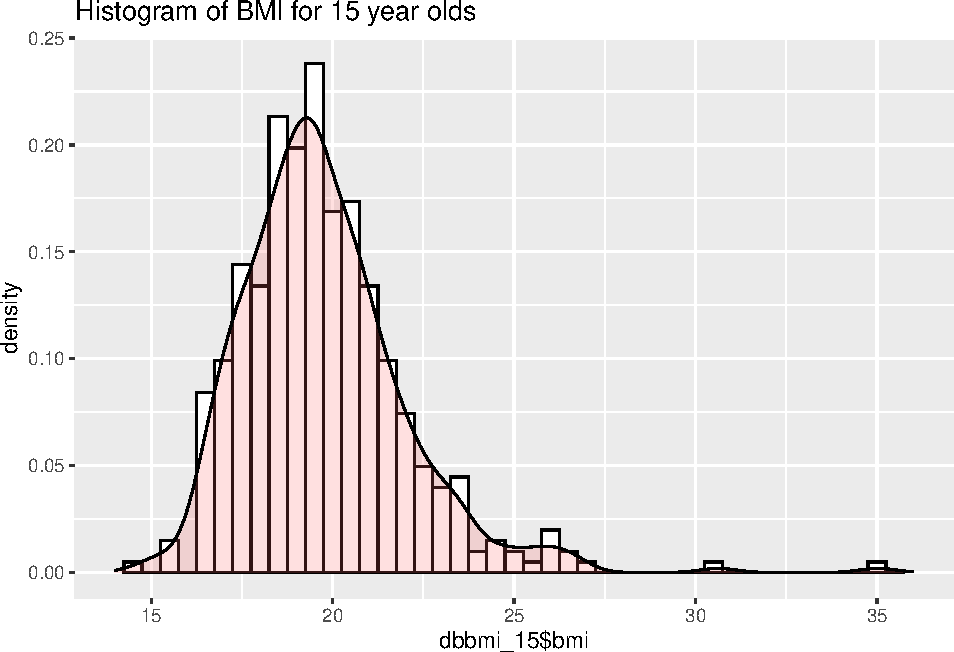
\includegraphics{assignment_q1_bmi_files/figure-latex/unnamed-chunk-1-2.pdf}

Experiment with the \texttt{nbins} parameter to find a visually
appealing and informative histogram. The goal is to have enough bins to
clearly see the distribution's shape without making it too noisy.

\hypertarget{b-fit-different-parametric-distributions-to-the-data-and-choose-an-appropriate-distribution-to-the-data.-justify-the-choice-of-the-distribution-by-explaining-what-you-have-done-and-why-you-select-this-specific-distribution.}{%
\subsubsection{(b) Fit different parametric distributions to the data
and choose an appropriate distribution to the data. Justify the choice
of the distribution by explaining what you have done and why you select
this specific
distribution.}\label{b-fit-different-parametric-distributions-to-the-data-and-choose-an-appropriate-distribution-to-the-data.-justify-the-choice-of-the-distribution-by-explaining-what-you-have-done-and-why-you-select-this-specific-distribution.}}

Next, we'll fit several parametric distributions to the data. Common
distributions for BMI data include the Normal, Log-Normal, and Gamma
distributions, among others. The \texttt{gamlss} package provides
functions to fit a wide range of distributions.

\begin{Shaded}
\begin{Highlighting}[]
\CommentTok{\# m1 is the model with the lowest AIC: list the best 6 fits:}
\CommentTok{\#m1 \textless{}{-} fitDist(bmi, type=c(\textquotesingle{}realplus\textquotesingle{}), data=dbbmi\_15, k=2)}
\CommentTok{\#m1$fit[1:6]}
\CommentTok{\#m1 \textless{}{-} fitDist(bmi, type=c(\textquotesingle{}realline\textquotesingle{}), data=dbbmi\_15, k=2)}
\CommentTok{\#m1$fit[1:6]}
\NormalTok{m1 }\OtherTok{\textless{}{-}} \FunctionTok{fitDist}\NormalTok{(bmi, }\AttributeTok{type=}\StringTok{\textquotesingle{}realAll\textquotesingle{}}\NormalTok{, }\AttributeTok{data=}\NormalTok{dbbmi\_15, }\AttributeTok{k=}\DecValTok{2}\NormalTok{)}
\end{Highlighting}
\end{Shaded}

\begin{verbatim}
##   |                                                                              |                                                                      |   0%  |                                                                              |=                                                                     |   2%  |                                                                              |===                                                                   |   4%  |                                                                              |====                                                                  |   6%  |                                                                              |=====                                                                 |   8%  |                                                                              |=======                                                               |  10%  |                                                                              |========                                                              |  12%  |                                                                              |==========                                                            |  14%  |                                                                              |===========                                                           |  16%  |                                                                              |============                                                          |  18%  |                                                                              |==============                                                        |  20%  |                                                                              |===============                                                       |  22%  |                                                                              |================                                                      |  24%  |                                                                              |==================                                                    |  25%  |                                                                              |===================                                                   |  27%  |                                                                              |=====================                                                 |  29%  |                                                                              |======================                                                |  31%  |                                                                              |=======================                                               |  33%  |                                                                              |=========================                                             |  35%  |                                                                              |==========================                                            |  37%  |                                                                              |===========================                                           |  39%  |                                                                              |=============================                                         |  41%  |                                                                              |==============================                                        |  43%  |                                                                              |================================                                      |  45%  |                                                                              |=================================                                     |  47%  |                                                                              |==================================                                    |  49%  |                                                                              |====================================                                  |  51%  |                                                                              |=====================================                                 |  53%  |                                                                              |======================================                                |  55%  |                                                                              |========================================                              |  57%  |                                                                              |=========================================                             |  59%  |                                                                              |===========================================                           |  61%  |                                                                              |============================================                          |  63%  |                                                                              |=============================================                         |  65%  |                                                                              |===============================================                       |  67%  |                                                                              |================================================                      |  69%  |                                                                              |=================================================                     |  71%  |                                                                              |===================================================                   |  73%  |                                                                              |====================================================                  |  75%  |                                                                              |======================================================                |  76%  |                                                                              |=======================================================               |  78%  |                                                                              |========================================================              |  80%  |                                                                              |==========================================================            |  82%  |                                                                              |===========================================================           |  84%  |                                                                              |============================================================          |  86%  |                                                                              |==============================================================        |  88%  |                                                                              |===============================================================       |  90%  |                                                                              |=================================================================     |  92%  |                                                                              |==================================================================    |  94%  |                                                                              |===================================================================   |  96%  |                                                                              |===================================================================== |  98%  |                                                                              |======================================================================| 100%
\end{verbatim}

\begin{Shaded}
\begin{Highlighting}[]
\NormalTok{m1}\SpecialCharTok{$}\NormalTok{fit[}\DecValTok{1}\SpecialCharTok{:}\DecValTok{6}\NormalTok{]}
\end{Highlighting}
\end{Shaded}

\begin{verbatim}
##   exGAUS    BCPEo     BCPE     BCTo      BCT      ST5 
## 1729.537 1729.731 1729.731 1729.992 1729.992 1730.401
\end{verbatim}

\begin{Shaded}
\begin{Highlighting}[]
\NormalTok{m1 }\OtherTok{\textless{}{-}} \FunctionTok{histDist}\NormalTok{(bmi, }\StringTok{"exGAUS"}\NormalTok{, }\AttributeTok{density=}\ConstantTok{TRUE}\NormalTok{, }\AttributeTok{line.col=}\FunctionTok{c}\NormalTok{(}\DecValTok{1}\NormalTok{,}\DecValTok{1}\NormalTok{), }\AttributeTok{line.ty=}\FunctionTok{c}\NormalTok{(}\DecValTok{1}\NormalTok{,}\DecValTok{2}\NormalTok{), }\AttributeTok{nbins=}\NormalTok{nbins, }\AttributeTok{data=}\NormalTok{dbbmi\_15)}
\end{Highlighting}
\end{Shaded}

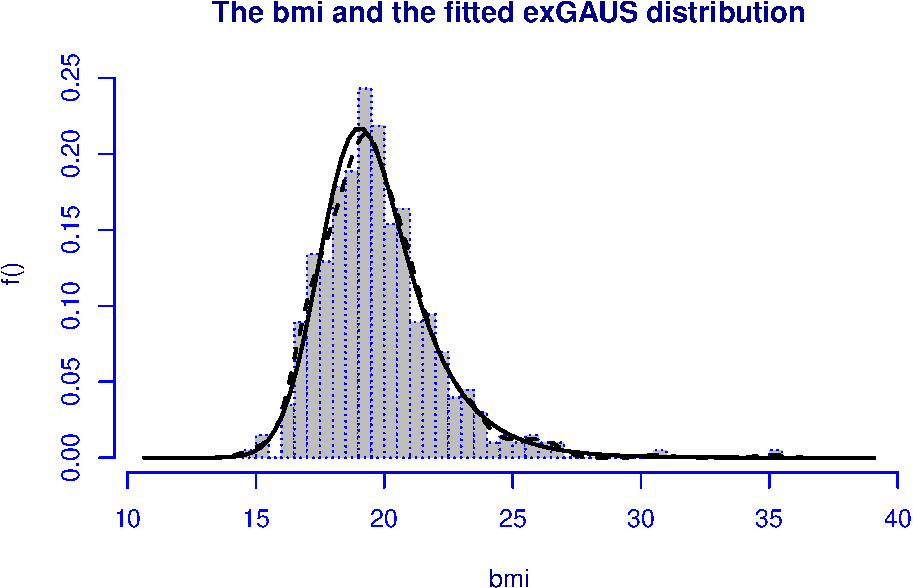
\includegraphics{assignment_q1_bmi_files/figure-latex/unnamed-chunk-3-1.pdf}

\begin{Shaded}
\begin{Highlighting}[]
\FunctionTok{plot}\NormalTok{(m1)}
\end{Highlighting}
\end{Shaded}

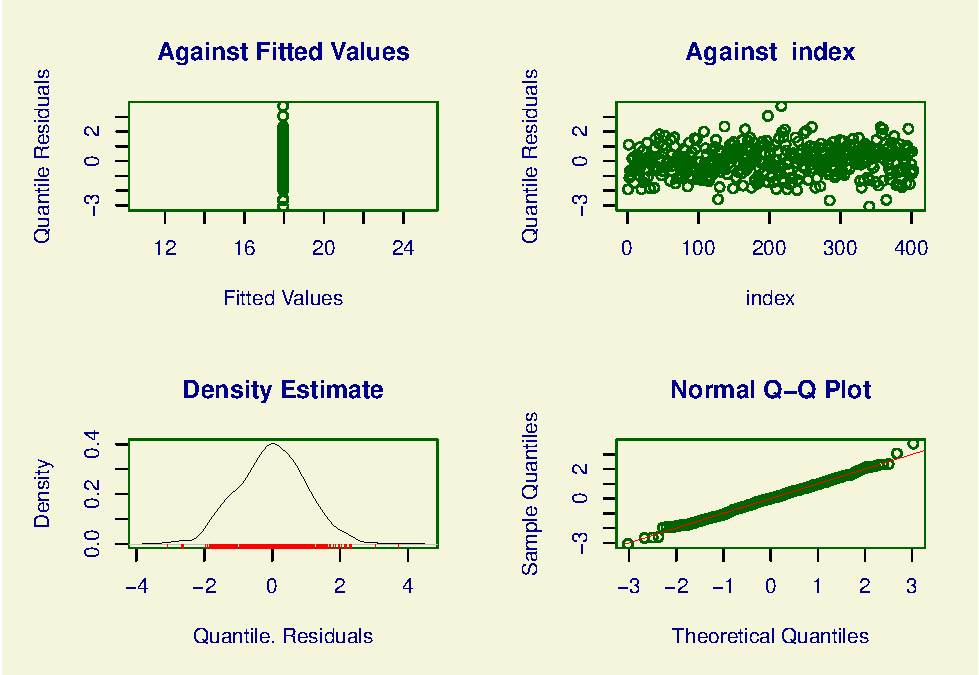
\includegraphics{assignment_q1_bmi_files/figure-latex/unnamed-chunk-3-2.pdf}

\begin{verbatim}
## ******************************************************************
##        Summary of the Quantile Residuals
##                            mean   =  -0.00222054 
##                        variance   =  1.005728 
##                coef. of skewness  =  0.05915047 
##                coef. of kurtosis  =  3.193805 
## Filliben correlation coefficient  =  0.9982076 
## ******************************************************************
\end{verbatim}

\begin{Shaded}
\begin{Highlighting}[]
\NormalTok{m2 }\OtherTok{\textless{}{-}} \FunctionTok{histDist}\NormalTok{(bmi, }\StringTok{"BCPEo"}\NormalTok{, }\AttributeTok{density=}\ConstantTok{TRUE}\NormalTok{, }\AttributeTok{line.col=}\FunctionTok{c}\NormalTok{(}\DecValTok{1}\NormalTok{,}\DecValTok{1}\NormalTok{), }\AttributeTok{line.ty=}\FunctionTok{c}\NormalTok{(}\DecValTok{1}\NormalTok{,}\DecValTok{2}\NormalTok{), }\AttributeTok{nbins=}\NormalTok{nbins, }\AttributeTok{data=}\NormalTok{dbbmi\_15)}
\end{Highlighting}
\end{Shaded}

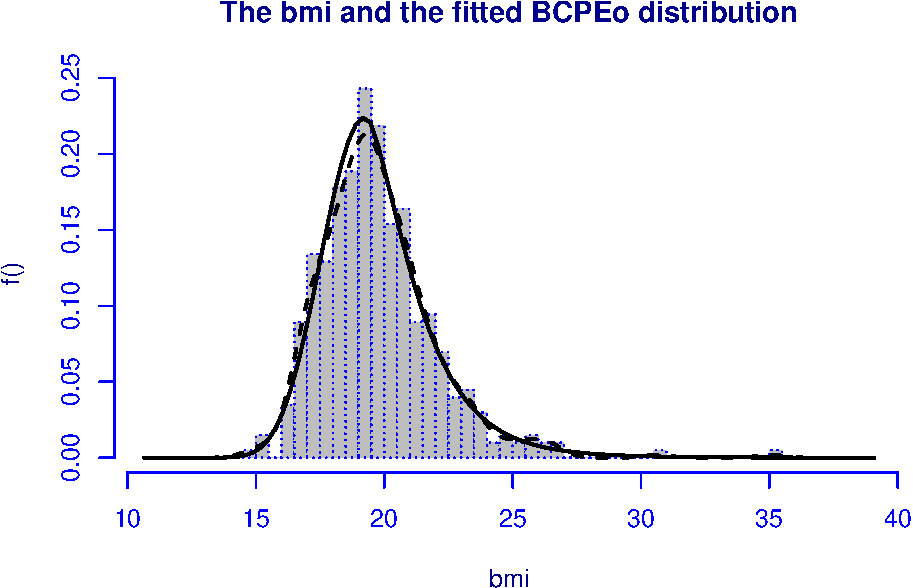
\includegraphics{assignment_q1_bmi_files/figure-latex/unnamed-chunk-3-3.pdf}

\begin{Shaded}
\begin{Highlighting}[]
\FunctionTok{plot}\NormalTok{(m2)}
\end{Highlighting}
\end{Shaded}

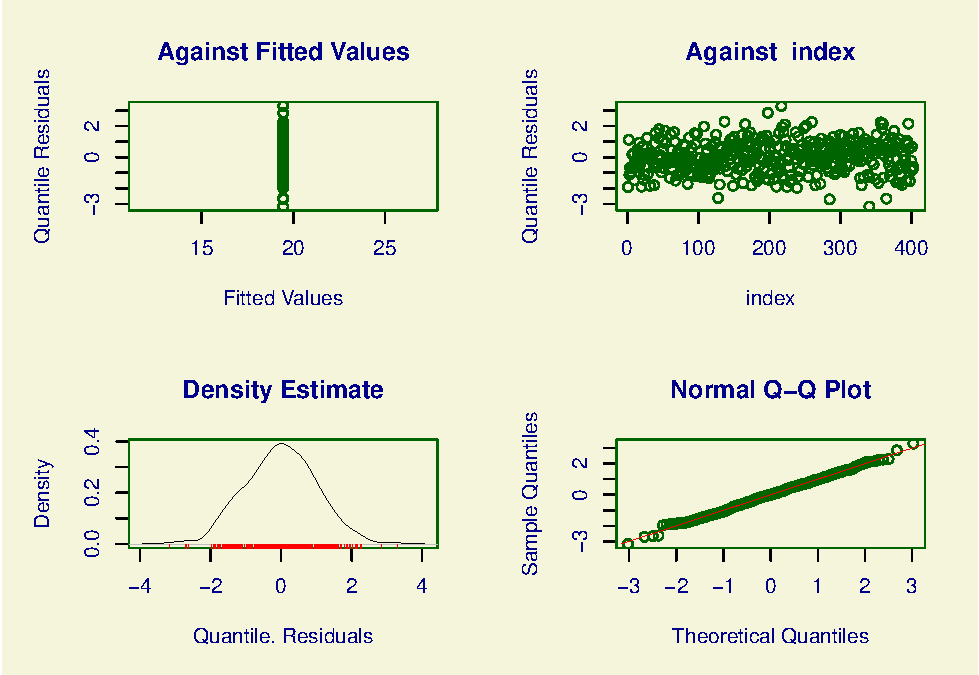
\includegraphics{assignment_q1_bmi_files/figure-latex/unnamed-chunk-3-4.pdf}

\begin{verbatim}
## ******************************************************************
##        Summary of the Quantile Residuals
##                            mean   =  -0.002539429 
##                        variance   =  1.00257 
##                coef. of skewness  =  -0.001697173 
##                coef. of kurtosis  =  2.997353 
## Filliben correlation coefficient  =  0.9988481 
## ******************************************************************
\end{verbatim}

\begin{Shaded}
\begin{Highlighting}[]
\NormalTok{m3 }\OtherTok{\textless{}{-}} \FunctionTok{histDist}\NormalTok{(bmi, }\StringTok{"BCPE"}\NormalTok{, }\AttributeTok{density=}\ConstantTok{TRUE}\NormalTok{, }\AttributeTok{line.col=}\FunctionTok{c}\NormalTok{(}\DecValTok{1}\NormalTok{,}\DecValTok{1}\NormalTok{), }\AttributeTok{line.ty=}\FunctionTok{c}\NormalTok{(}\DecValTok{1}\NormalTok{,}\DecValTok{2}\NormalTok{), }\AttributeTok{nbins=}\NormalTok{nbins, }\AttributeTok{data=}\NormalTok{dbbmi\_15)}
\end{Highlighting}
\end{Shaded}

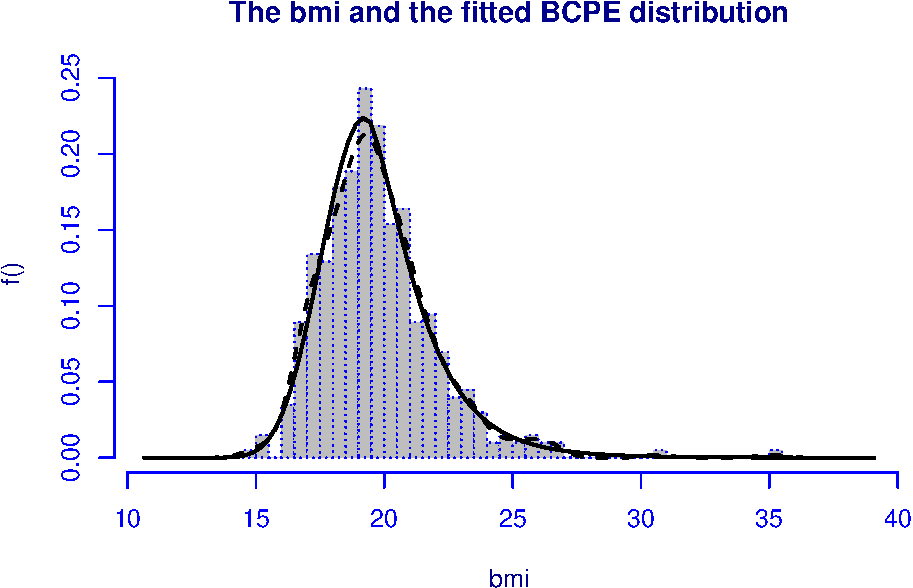
\includegraphics{assignment_q1_bmi_files/figure-latex/unnamed-chunk-3-5.pdf}

\begin{Shaded}
\begin{Highlighting}[]
\FunctionTok{plot}\NormalTok{(m3)}
\end{Highlighting}
\end{Shaded}

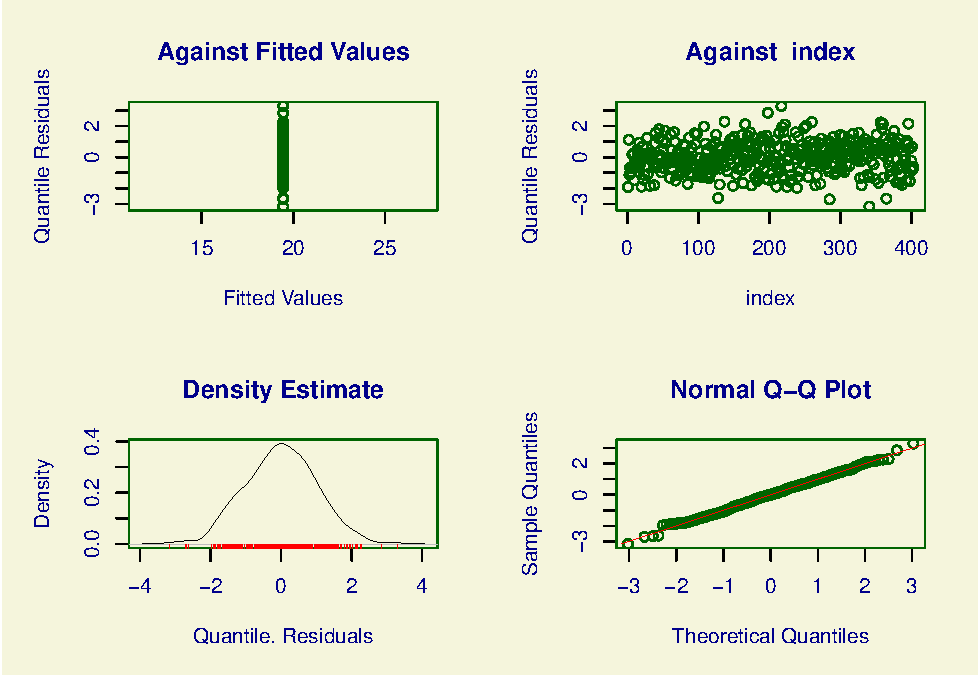
\includegraphics{assignment_q1_bmi_files/figure-latex/unnamed-chunk-3-6.pdf}

\begin{verbatim}
## ******************************************************************
##        Summary of the Quantile Residuals
##                            mean   =  -0.002537045 
##                        variance   =  1.00257 
##                coef. of skewness  =  -0.001697852 
##                coef. of kurtosis  =  2.997391 
## Filliben correlation coefficient  =  0.9988481 
## ******************************************************************
\end{verbatim}

\begin{Shaded}
\begin{Highlighting}[]
\NormalTok{m1 }\OtherTok{\textless{}{-}} \FunctionTok{gamlss}\NormalTok{(bmi}\SpecialCharTok{\textasciitilde{}}\DecValTok{1}\NormalTok{, }\AttributeTok{family=}\NormalTok{NO, }\AttributeTok{data=}\NormalTok{dbbmi\_15)}
\end{Highlighting}
\end{Shaded}

\begin{verbatim}
## GAMLSS-RS iteration 1: Global Deviance = 1803.044 
## GAMLSS-RS iteration 2: Global Deviance = 1803.044
\end{verbatim}

\begin{Shaded}
\begin{Highlighting}[]
\NormalTok{c1 }\OtherTok{\textless{}{-}} \FunctionTok{chooseDist}\NormalTok{(m1, }\AttributeTok{type=}\StringTok{\textquotesingle{}realAll\textquotesingle{}}\NormalTok{, }\AttributeTok{data=}\NormalTok{dbbmi\_15, }\AttributeTok{parallel=}\StringTok{"snow"}\NormalTok{, }\AttributeTok{ncpus=}\DecValTok{4}\NormalTok{)}
\end{Highlighting}
\end{Shaded}

\begin{verbatim}
## minimum GAIC(k= 2 ) family: exGAUS 
## minimum GAIC(k= 3.84 ) family: exGAUS 
## minimum GAIC(k= 6 ) family: exGAUS
\end{verbatim}

\begin{Shaded}
\begin{Highlighting}[]
\NormalTok{c1}
\end{Highlighting}
\end{Shaded}

\begin{verbatim}
##                 2     3.84        6
## NO       1807.044 1810.724 1815.044
## GU       2117.531 2121.211 2125.531
## RG       1733.816 1737.496 1741.816
## LO       1761.949 1765.629 1769.949
## NET      1759.479 1763.159 1767.479
## TF       1756.536 1762.056 1768.536
## TF2      1756.537 1762.057 1768.537
## PE       1766.779 1772.299 1778.779
## PE2      1766.783 1772.303 1778.783
## SN1      1809.044 1814.564 1821.044
## SN2      1755.128 1760.648 1767.128
## exGAUS   1729.537 1735.057 1741.537
## SHASH    1735.278 1742.638 1751.278
## SHASHo   1740.368 1747.728 1756.368
## SHASHo2  1740.098 1747.458 1756.098
## EGB2     1734.237 1741.597 1750.237
## JSU      1731.709 1739.069 1747.709
## JSUo     1739.039 1746.399 1755.039
## SEP1     1742.582 1749.942 1758.582
## SEP2     1749.584 1756.944 1765.584
## SEP3     1742.365 1749.725 1758.365
## SEP4     1732.778 1740.138 1748.778
## ST1      1734.015 1741.375 1750.015
## ST2      1737.021 1744.381 1753.021
## ST3      1735.795 1743.155 1751.795
## ST4      1733.081 1740.441 1749.081
## ST5      1732.808 1740.168 1748.808
## SST      1735.770 1743.130 1751.770
## GT       1757.541 1764.901 1773.541
## EXP      3212.376 3214.216 3216.376
## GA       1772.064 1775.744 1780.064
## IG       1759.441 1763.121 1767.441
## LOGNO    1758.605 1762.285 1766.605
## LOGNO2   1758.605 1762.285 1766.605
## WEI      1966.621 1970.301 1974.621
## WEI2     2373.622 2377.302 2381.622
## WEI3     1966.621 1970.301 1974.621
## IGAMMA   1748.193 1751.873 1756.193
## PARETO2  3251.903 3255.583 3259.903
## PARETO2o 3222.313 3225.993 3230.313
## GP       3251.903 3255.583 3259.903
## BCCG     1730.663 1736.183 1742.663
## BCCGo    1730.663 1736.183 1742.663
## GG       1732.317 1737.837 1744.317
## GIG      1750.193 1755.713 1762.193
## LNO      1758.605 1762.285 1766.605
## BCTo     1729.992 1737.352 1745.992
## BCT      1729.992 1737.352 1745.992
## BCPEo    1729.731 1737.091 1745.731
## BCPE     1729.731 1737.091 1745.731
## GB2      1732.204 1739.564 1748.204
\end{verbatim}

\hypertarget{best-fit-is-bccg}{%
\paragraph{Best fit is BCCG}\label{best-fit-is-bccg}}

\begin{Shaded}
\begin{Highlighting}[]
\CommentTok{\# Best fit is BCCG}
\NormalTok{m1 }\OtherTok{\textless{}{-}} \FunctionTok{histDist}\NormalTok{(bmi, }\StringTok{"BCCG"}\NormalTok{, }\AttributeTok{density=}\ConstantTok{TRUE}\NormalTok{, }\AttributeTok{line.col=}\FunctionTok{c}\NormalTok{(}\DecValTok{1}\NormalTok{,}\DecValTok{1}\NormalTok{), }\AttributeTok{line.ty=}\FunctionTok{c}\NormalTok{(}\DecValTok{1}\NormalTok{,}\DecValTok{2}\NormalTok{), }\AttributeTok{nbins=}\NormalTok{nbins, }\AttributeTok{data=}\NormalTok{dbbmi\_15)}
\end{Highlighting}
\end{Shaded}

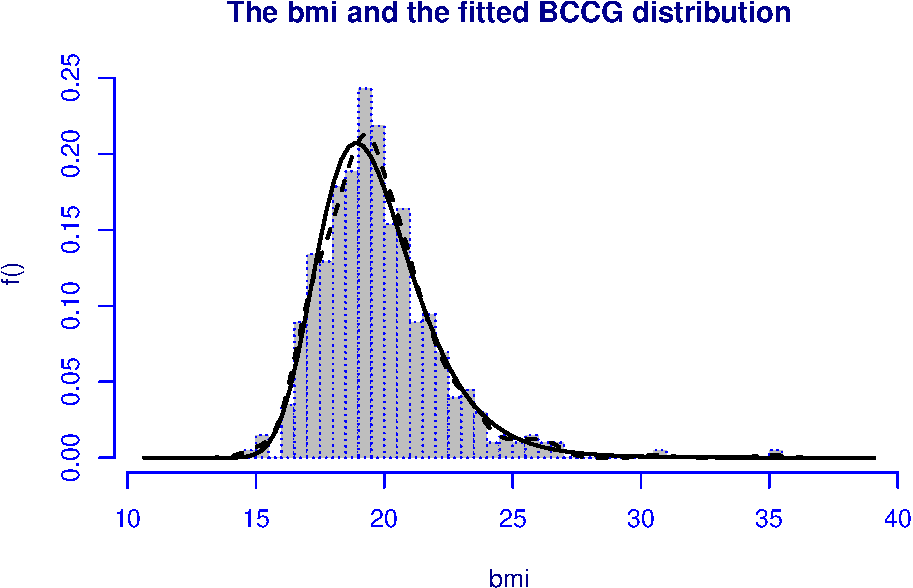
\includegraphics{assignment_q1_bmi_files/figure-latex/unnamed-chunk-5-1.pdf}

\begin{Shaded}
\begin{Highlighting}[]
\FunctionTok{plot}\NormalTok{(m1)}
\end{Highlighting}
\end{Shaded}

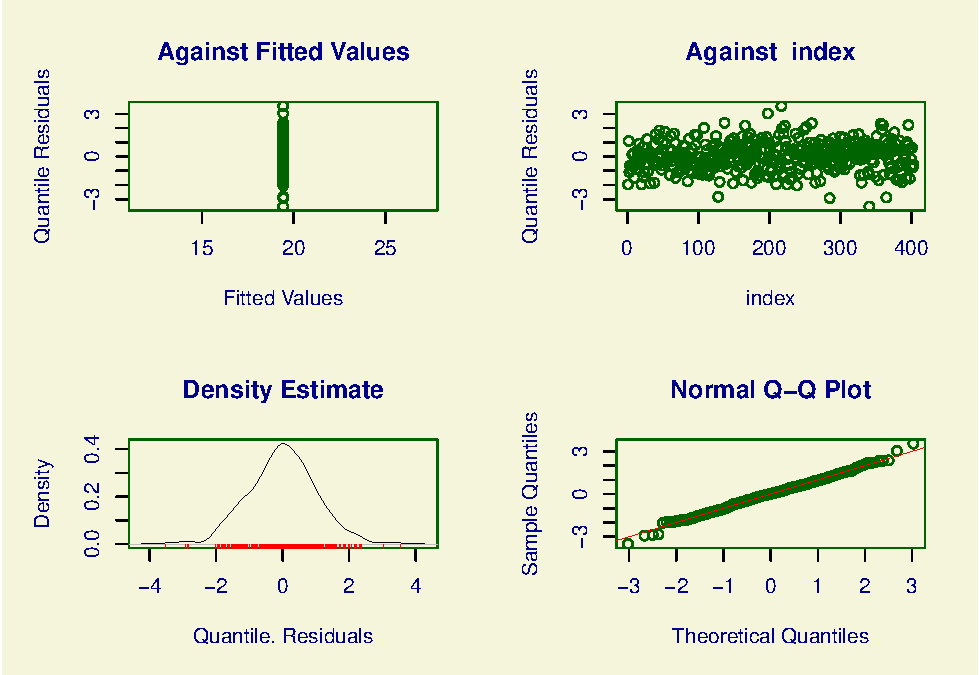
\includegraphics{assignment_q1_bmi_files/figure-latex/unnamed-chunk-5-2.pdf}

\begin{verbatim}
## ******************************************************************
##        Summary of the Quantile Residuals
##                            mean   =  1.683958e-07 
##                        variance   =  1.002488 
##                coef. of skewness  =  -0.0312982 
##                coef. of kurtosis  =  3.44508 
## Filliben correlation coefficient  =  0.9976684 
## ******************************************************************
\end{verbatim}

\begin{Shaded}
\begin{Highlighting}[]
\NormalTok{m2 }\OtherTok{\textless{}{-}} \FunctionTok{histDist}\NormalTok{(bmi, }\StringTok{"TF"}\NormalTok{, }\AttributeTok{density=}\ConstantTok{TRUE}\NormalTok{, }\AttributeTok{line.col=}\FunctionTok{c}\NormalTok{(}\DecValTok{1}\NormalTok{,}\DecValTok{1}\NormalTok{), }\AttributeTok{line.ty=}\FunctionTok{c}\NormalTok{(}\DecValTok{1}\NormalTok{,}\DecValTok{2}\NormalTok{), }\AttributeTok{nbins=}\NormalTok{nbins, }\AttributeTok{data=}\NormalTok{dbbmi\_15)}
\end{Highlighting}
\end{Shaded}

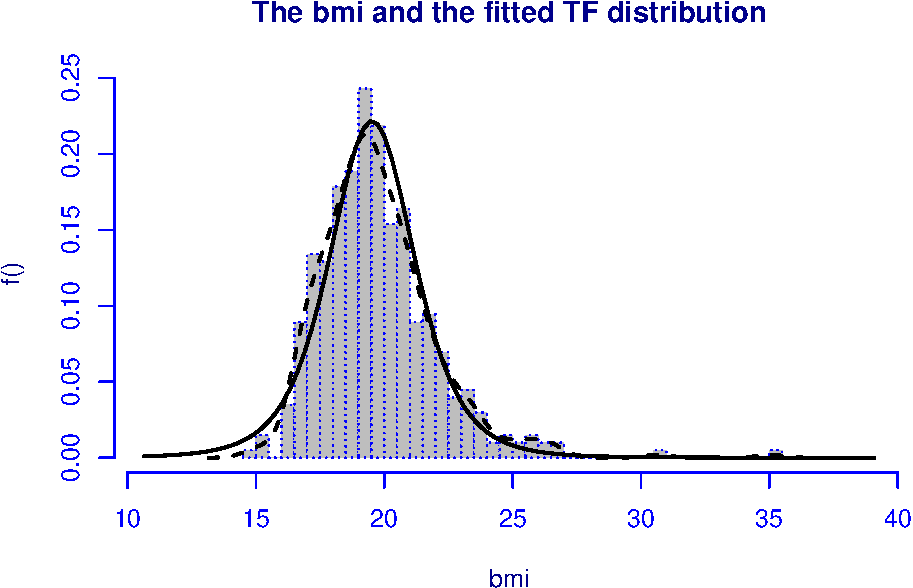
\includegraphics{assignment_q1_bmi_files/figure-latex/unnamed-chunk-5-3.pdf}

\begin{Shaded}
\begin{Highlighting}[]
\FunctionTok{plot}\NormalTok{(m2)}
\end{Highlighting}
\end{Shaded}

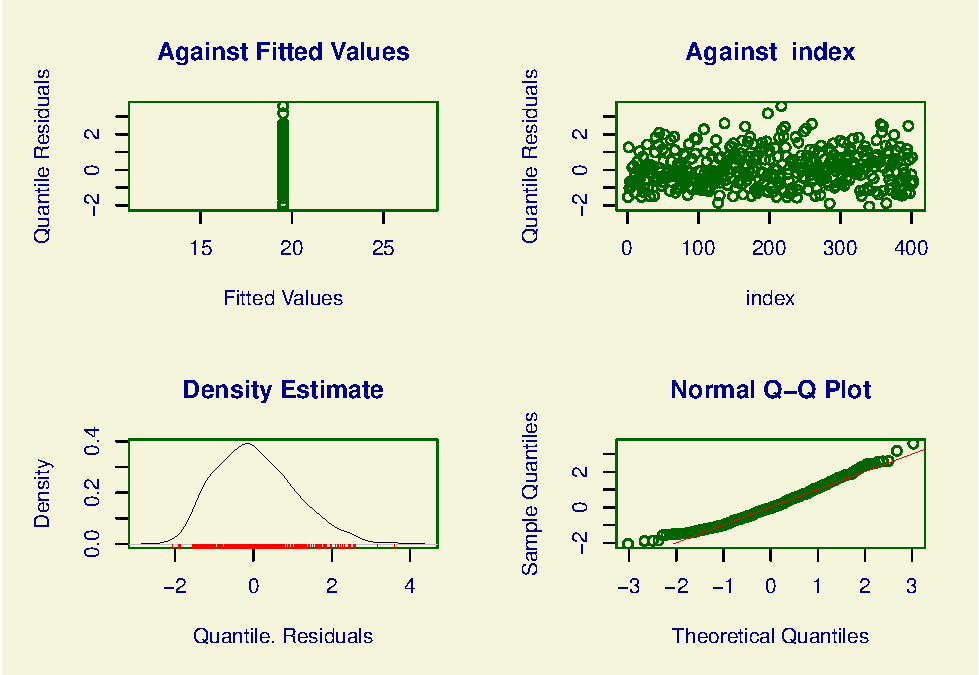
\includegraphics{assignment_q1_bmi_files/figure-latex/unnamed-chunk-5-4.pdf}

\begin{verbatim}
## ******************************************************************
##        Summary of the Quantile Residuals
##                            mean   =  0.06736512 
##                        variance   =  0.9980666 
##                coef. of skewness  =  0.4946411 
##                coef. of kurtosis  =  2.93465 
## Filliben correlation coefficient  =  0.990266 
## ******************************************************************
\end{verbatim}

\begin{Shaded}
\begin{Highlighting}[]
\NormalTok{m3 }\OtherTok{\textless{}{-}} \FunctionTok{histDist}\NormalTok{(bmi, }\StringTok{"exGAUS"}\NormalTok{, }\AttributeTok{density=}\ConstantTok{TRUE}\NormalTok{, }\AttributeTok{line.col=}\FunctionTok{c}\NormalTok{(}\DecValTok{1}\NormalTok{,}\DecValTok{1}\NormalTok{), }\AttributeTok{line.ty=}\FunctionTok{c}\NormalTok{(}\DecValTok{1}\NormalTok{,}\DecValTok{2}\NormalTok{), }\AttributeTok{nbins=}\NormalTok{nbins, }\AttributeTok{data=}\NormalTok{dbbmi\_15)}
\end{Highlighting}
\end{Shaded}

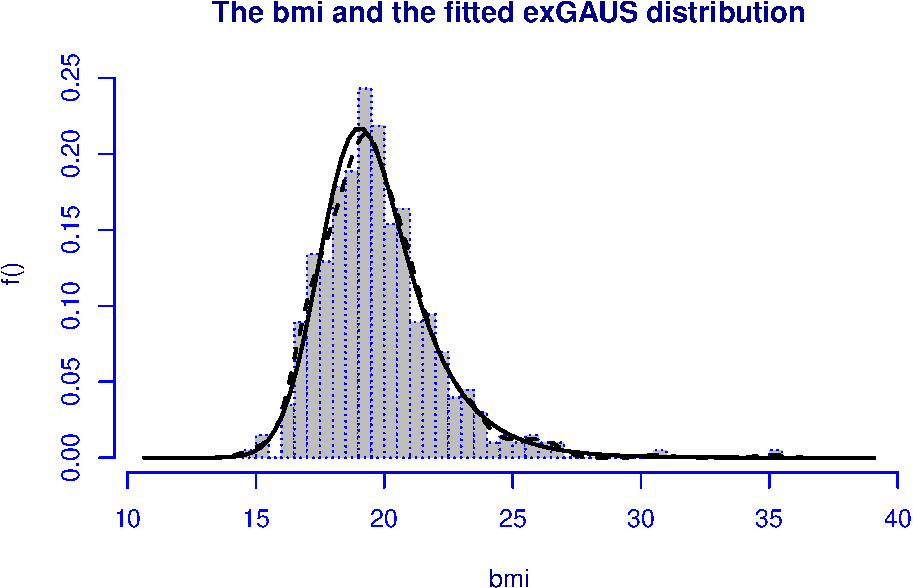
\includegraphics{assignment_q1_bmi_files/figure-latex/unnamed-chunk-5-5.pdf}

\begin{Shaded}
\begin{Highlighting}[]
\FunctionTok{plot}\NormalTok{(m3)}
\end{Highlighting}
\end{Shaded}

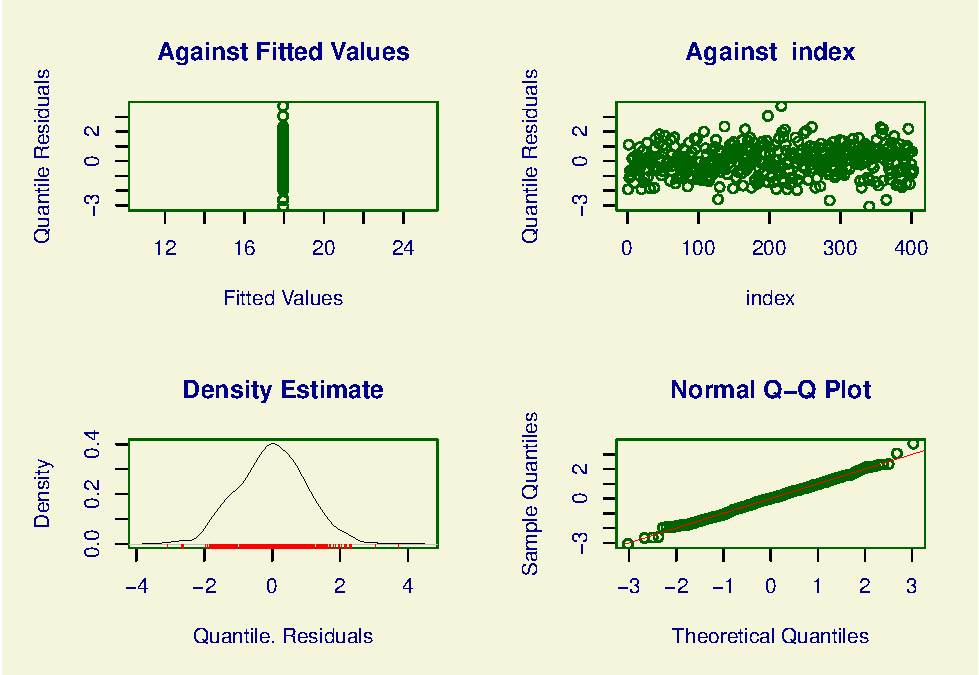
\includegraphics{assignment_q1_bmi_files/figure-latex/unnamed-chunk-5-6.pdf}

\begin{verbatim}
## ******************************************************************
##        Summary of the Quantile Residuals
##                            mean   =  -0.00222054 
##                        variance   =  1.005728 
##                coef. of skewness  =  0.05915047 
##                coef. of kurtosis  =  3.193805 
## Filliben correlation coefficient  =  0.9982076 
## ******************************************************************
\end{verbatim}

\begin{Shaded}
\begin{Highlighting}[]
\FunctionTok{plot}\NormalTok{(}\ControlFlowTok{function}\NormalTok{(x) }\FunctionTok{dJSU}\NormalTok{(x, }\AttributeTok{mu=}\FloatTok{16.8475}\NormalTok{, }\AttributeTok{sigma=}\FloatTok{1.7560}\NormalTok{, }\AttributeTok{nu=}\FloatTok{2.439}\NormalTok{, }\AttributeTok{tau=}\FloatTok{2.6890}\NormalTok{), }\DecValTok{10}\NormalTok{, }\DecValTok{25}\NormalTok{, }\AttributeTok{main =} \StringTok{"The JSU  density mu=16.8475, sigma=0.7560, nu=2.439, tau=0.6890"}\NormalTok{)}
\end{Highlighting}
\end{Shaded}

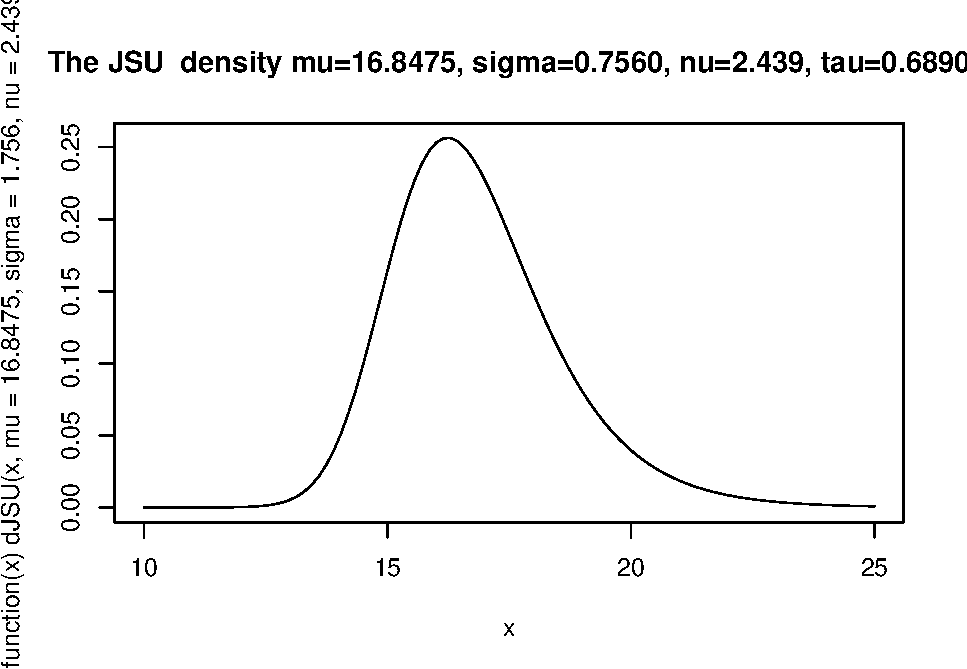
\includegraphics{assignment_q1_bmi_files/figure-latex/unnamed-chunk-6-1.pdf}

\begin{Shaded}
\begin{Highlighting}[]
\CommentTok{\#print(dJSU(x, mu=16.8475, sigma=1.7560, nu=2.439, tau=2.742))}
\end{Highlighting}
\end{Shaded}

\begin{Shaded}
\begin{Highlighting}[]
\CommentTok{\# Fit different distributions}
\NormalTok{fit\_bccg }\OtherTok{\textless{}{-}} \FunctionTok{gamlss}\NormalTok{(bmi15 }\SpecialCharTok{\textasciitilde{}} \DecValTok{1}\NormalTok{, }\AttributeTok{family=}\NormalTok{BCCG)}
\end{Highlighting}
\end{Shaded}

\begin{verbatim}
## GAMLSS-RS iteration 1: Global Deviance = 1732.959 
## GAMLSS-RS iteration 2: Global Deviance = 1725.178 
## GAMLSS-RS iteration 3: Global Deviance = 1724.682 
## GAMLSS-RS iteration 4: Global Deviance = 1724.664 
## GAMLSS-RS iteration 5: Global Deviance = 1724.663
\end{verbatim}

\begin{Shaded}
\begin{Highlighting}[]
\NormalTok{fit\_jsu }\OtherTok{\textless{}{-}} \FunctionTok{gamlss}\NormalTok{(bmi15 }\SpecialCharTok{\textasciitilde{}} \DecValTok{1}\NormalTok{, }\AttributeTok{family=}\NormalTok{JSU)}
\end{Highlighting}
\end{Shaded}

\begin{verbatim}
## GAMLSS-RS iteration 1: Global Deviance = 1759.315 
## GAMLSS-RS iteration 2: Global Deviance = 1741.358 
## GAMLSS-RS iteration 3: Global Deviance = 1733.024 
## GAMLSS-RS iteration 4: Global Deviance = 1728.984 
## GAMLSS-RS iteration 5: Global Deviance = 1726.744 
## GAMLSS-RS iteration 6: Global Deviance = 1725.473 
## GAMLSS-RS iteration 7: Global Deviance = 1724.745 
## GAMLSS-RS iteration 8: Global Deviance = 1724.328 
## GAMLSS-RS iteration 9: Global Deviance = 1724.085 
## GAMLSS-RS iteration 10: Global Deviance = 1723.94 
## GAMLSS-RS iteration 11: Global Deviance = 1723.855 
## GAMLSS-RS iteration 12: Global Deviance = 1723.801 
## GAMLSS-RS iteration 13: Global Deviance = 1723.767 
## GAMLSS-RS iteration 14: Global Deviance = 1723.746 
## GAMLSS-RS iteration 15: Global Deviance = 1723.732 
## GAMLSS-RS iteration 16: Global Deviance = 1723.723 
## GAMLSS-RS iteration 17: Global Deviance = 1723.717 
## GAMLSS-RS iteration 18: Global Deviance = 1723.713 
## GAMLSS-RS iteration 19: Global Deviance = 1723.711 
## GAMLSS-RS iteration 20: Global Deviance = 1723.709
\end{verbatim}

\begin{Shaded}
\begin{Highlighting}[]
\NormalTok{fit\_tf }\OtherTok{\textless{}{-}} \FunctionTok{gamlss}\NormalTok{(bmi15 }\SpecialCharTok{\textasciitilde{}} \DecValTok{1}\NormalTok{, }\AttributeTok{family=}\NormalTok{TF)}
\end{Highlighting}
\end{Shaded}

\begin{verbatim}
## GAMLSS-RS iteration 1: Global Deviance = 1754.007 
## GAMLSS-RS iteration 2: Global Deviance = 1751.186 
## GAMLSS-RS iteration 3: Global Deviance = 1750.66 
## GAMLSS-RS iteration 4: Global Deviance = 1750.56 
## GAMLSS-RS iteration 5: Global Deviance = 1750.541 
## GAMLSS-RS iteration 6: Global Deviance = 1750.537 
## GAMLSS-RS iteration 7: Global Deviance = 1750.536
\end{verbatim}

\begin{Shaded}
\begin{Highlighting}[]
\NormalTok{fit\_lognorm }\OtherTok{\textless{}{-}} \FunctionTok{gamlss}\NormalTok{(bmi15 }\SpecialCharTok{\textasciitilde{}} \DecValTok{1}\NormalTok{, }\AttributeTok{family=}\NormalTok{LOGNO)}
\end{Highlighting}
\end{Shaded}

\begin{verbatim}
## GAMLSS-RS iteration 1: Global Deviance = 1754.605 
## GAMLSS-RS iteration 2: Global Deviance = 1754.605
\end{verbatim}

\begin{Shaded}
\begin{Highlighting}[]
\NormalTok{fit\_lo }\OtherTok{\textless{}{-}} \FunctionTok{gamlss}\NormalTok{(bmi15 }\SpecialCharTok{\textasciitilde{}} \DecValTok{1}\NormalTok{, }\AttributeTok{family=}\NormalTok{LO)}
\end{Highlighting}
\end{Shaded}

\begin{verbatim}
## GAMLSS-RS iteration 1: Global Deviance = 1758.388 
## GAMLSS-RS iteration 2: Global Deviance = 1757.949 
## GAMLSS-RS iteration 3: Global Deviance = 1757.949
\end{verbatim}

\begin{Shaded}
\begin{Highlighting}[]
\NormalTok{fit\_pe }\OtherTok{\textless{}{-}} \FunctionTok{gamlss}\NormalTok{(bmi15 }\SpecialCharTok{\textasciitilde{}} \DecValTok{1}\NormalTok{, }\AttributeTok{family=}\NormalTok{PE)}
\end{Highlighting}
\end{Shaded}

\begin{verbatim}
## GAMLSS-RS iteration 1: Global Deviance = 1761.569 
## GAMLSS-RS iteration 2: Global Deviance = 1760.787 
## GAMLSS-RS iteration 3: Global Deviance = 1760.779 
## GAMLSS-RS iteration 4: Global Deviance = 1760.779
\end{verbatim}

\begin{Shaded}
\begin{Highlighting}[]
\NormalTok{fit\_gamma }\OtherTok{\textless{}{-}} \FunctionTok{gamlss}\NormalTok{(bmi15 }\SpecialCharTok{\textasciitilde{}} \DecValTok{1}\NormalTok{, }\AttributeTok{family=}\NormalTok{GA)}
\end{Highlighting}
\end{Shaded}

\begin{verbatim}
## GAMLSS-RS iteration 1: Global Deviance = 1768.064 
## GAMLSS-RS iteration 2: Global Deviance = 1768.064
\end{verbatim}

\begin{Shaded}
\begin{Highlighting}[]
\NormalTok{fit\_norm }\OtherTok{\textless{}{-}} \FunctionTok{gamlss}\NormalTok{(bmi15 }\SpecialCharTok{\textasciitilde{}} \DecValTok{1}\NormalTok{, }\AttributeTok{family=}\NormalTok{NO)}
\end{Highlighting}
\end{Shaded}

\begin{verbatim}
## GAMLSS-RS iteration 1: Global Deviance = 1803.044 
## GAMLSS-RS iteration 2: Global Deviance = 1803.044
\end{verbatim}

\begin{Shaded}
\begin{Highlighting}[]
\NormalTok{fit\_wei }\OtherTok{\textless{}{-}} \FunctionTok{gamlss}\NormalTok{(bmi15 }\SpecialCharTok{\textasciitilde{}} \DecValTok{1}\NormalTok{, }\AttributeTok{family=}\NormalTok{WEI)}
\end{Highlighting}
\end{Shaded}

\begin{verbatim}
## GAMLSS-RS iteration 1: Global Deviance = 2065.919 
## GAMLSS-RS iteration 2: Global Deviance = 1962.633 
## GAMLSS-RS iteration 3: Global Deviance = 1962.621 
## GAMLSS-RS iteration 4: Global Deviance = 1962.621
\end{verbatim}

\begin{Shaded}
\begin{Highlighting}[]
\NormalTok{fit\_gu }\OtherTok{\textless{}{-}} \FunctionTok{gamlss}\NormalTok{(bmi15 }\SpecialCharTok{\textasciitilde{}} \DecValTok{1}\NormalTok{, }\AttributeTok{family=}\NormalTok{GU)}
\end{Highlighting}
\end{Shaded}

\begin{verbatim}
## GAMLSS-RS iteration 1: Global Deviance = 2430.46 
## GAMLSS-RS iteration 2: Global Deviance = 2115.898 
## GAMLSS-RS iteration 3: Global Deviance = 2113.566 
## GAMLSS-RS iteration 4: Global Deviance = 2113.537 
## GAMLSS-RS iteration 5: Global Deviance = 2113.534 
## GAMLSS-RS iteration 6: Global Deviance = 2113.533 
## GAMLSS-RS iteration 7: Global Deviance = 2113.531 
## GAMLSS-RS iteration 8: Global Deviance = 2113.531
\end{verbatim}

\begin{Shaded}
\begin{Highlighting}[]
\NormalTok{fit\_exp }\OtherTok{\textless{}{-}} \FunctionTok{gamlss}\NormalTok{(bmi15 }\SpecialCharTok{\textasciitilde{}} \DecValTok{1}\NormalTok{, }\AttributeTok{family=}\NormalTok{EXP)}
\end{Highlighting}
\end{Shaded}

\begin{verbatim}
## GAMLSS-RS iteration 1: Global Deviance = 3210.376 
## GAMLSS-RS iteration 2: Global Deviance = 3210.376
\end{verbatim}

\begin{Shaded}
\begin{Highlighting}[]
\NormalTok{fit\_lg }\OtherTok{\textless{}{-}} \FunctionTok{gamlss}\NormalTok{(bmi15 }\SpecialCharTok{\textasciitilde{}} \DecValTok{1}\NormalTok{, }\AttributeTok{family=}\NormalTok{LG)}
\end{Highlighting}
\end{Shaded}

\begin{verbatim}
## GAMLSS-RS iteration 1: Global Deviance = 3794.267 
## GAMLSS-RS iteration 2: Global Deviance = 196714 
## GAMLSS-RS iteration 3: Global Deviance = 156994.3 
## GAMLSS-RS iteration 4: Global Deviance = 117274.7 
## GAMLSS-RS iteration 5: Global Deviance = 77557.7 
## GAMLSS-RS iteration 6: Global Deviance = 37876.95 
## GAMLSS-RS iteration 7: Global Deviance = 3792.951 
## GAMLSS-RS iteration 8: Global Deviance = 218029.3 
## GAMLSS-RS iteration 9: Global Deviance = 178309.6 
## GAMLSS-RS iteration 10: Global Deviance = 138589.9 
## GAMLSS-RS iteration 11: Global Deviance = 98870.84 
## GAMLSS-RS iteration 12: Global Deviance = 59160.25 
## GAMLSS-RS iteration 13: Global Deviance = 19593.09 
## GAMLSS-RS iteration 14: Global Deviance = 3790.757 
## GAMLSS-RS iteration 15: Global Deviance = 235692.1 
## GAMLSS-RS iteration 16: Global Deviance = 195972.3 
## GAMLSS-RS iteration 17: Global Deviance = 156252.6 
## GAMLSS-RS iteration 18: Global Deviance = 116533.1 
## GAMLSS-RS iteration 19: Global Deviance = 76816.22 
## GAMLSS-RS iteration 20: Global Deviance = 37137.54
\end{verbatim}

\begin{Shaded}
\begin{Highlighting}[]
\NormalTok{models }\OtherTok{\textless{}{-}} \FunctionTok{list}\NormalTok{(fit\_jsu, fit\_tf, fit\_lognorm, fit\_lo, fit\_pe, fit\_gamma, fit\_norm, fit\_wei, fit\_gu, fit\_exp, fit\_lg)}

\CommentTok{\# Compare models}
\NormalTok{aic\_values }\OtherTok{\textless{}{-}} \FunctionTok{sapply}\NormalTok{(models, AIC)}
\FunctionTok{print}\NormalTok{(aic\_values)}
\end{Highlighting}
\end{Shaded}

\begin{verbatim}
##  [1]  1731.709  1756.536  1758.605  1761.949  1766.779  1772.064  1807.044
##  [8]  1966.621  2117.531  3212.376 37139.545
\end{verbatim}

\begin{Shaded}
\begin{Highlighting}[]
\CommentTok{\# Select the model with the lowest AIC}
\NormalTok{selected\_model }\OtherTok{\textless{}{-}}\NormalTok{ models[[}\FunctionTok{which.min}\NormalTok{(aic\_values)]]}
\NormalTok{selected\_model }\OtherTok{\textless{}{-}} \FunctionTok{histDist}\NormalTok{(dbbmi\_15}\SpecialCharTok{$}\NormalTok{bmi, }\StringTok{"JSU"}\NormalTok{, }\AttributeTok{density=}\ConstantTok{TRUE}\NormalTok{, }\AttributeTok{line.col=}\FunctionTok{c}\NormalTok{(}\DecValTok{1}\NormalTok{,}\DecValTok{1}\NormalTok{), }\AttributeTok{line.ty=}\FunctionTok{c}\NormalTok{(}\DecValTok{1}\NormalTok{,}\DecValTok{2}\NormalTok{))}
\end{Highlighting}
\end{Shaded}

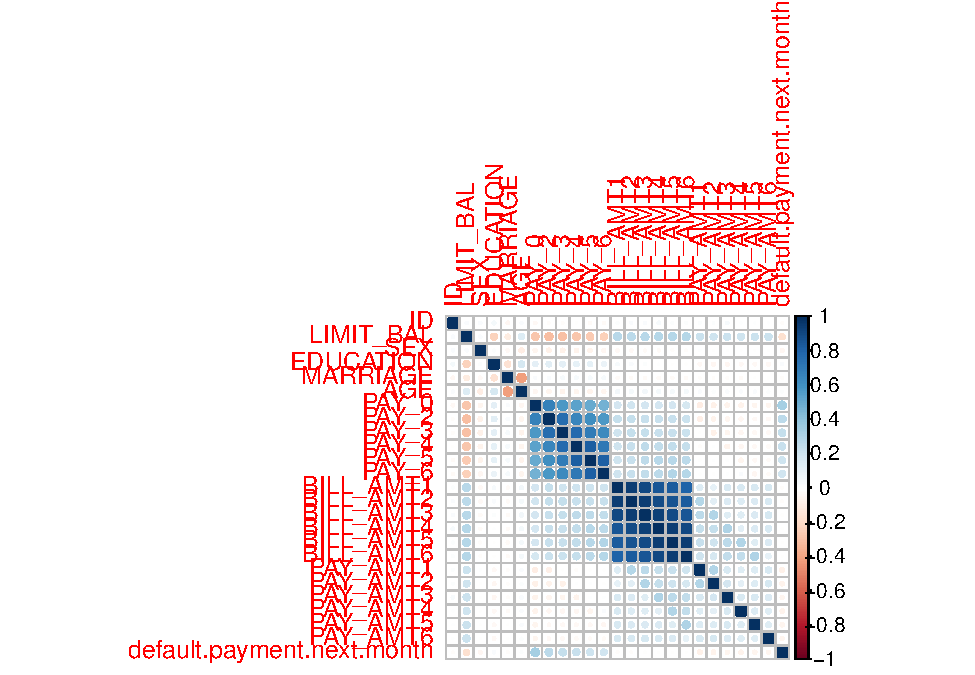
\includegraphics{assignment_q1_bmi_files/figure-latex/unnamed-chunk-8-1.pdf}

\begin{Shaded}
\begin{Highlighting}[]
\FunctionTok{plot}\NormalTok{(selected\_model)}
\end{Highlighting}
\end{Shaded}

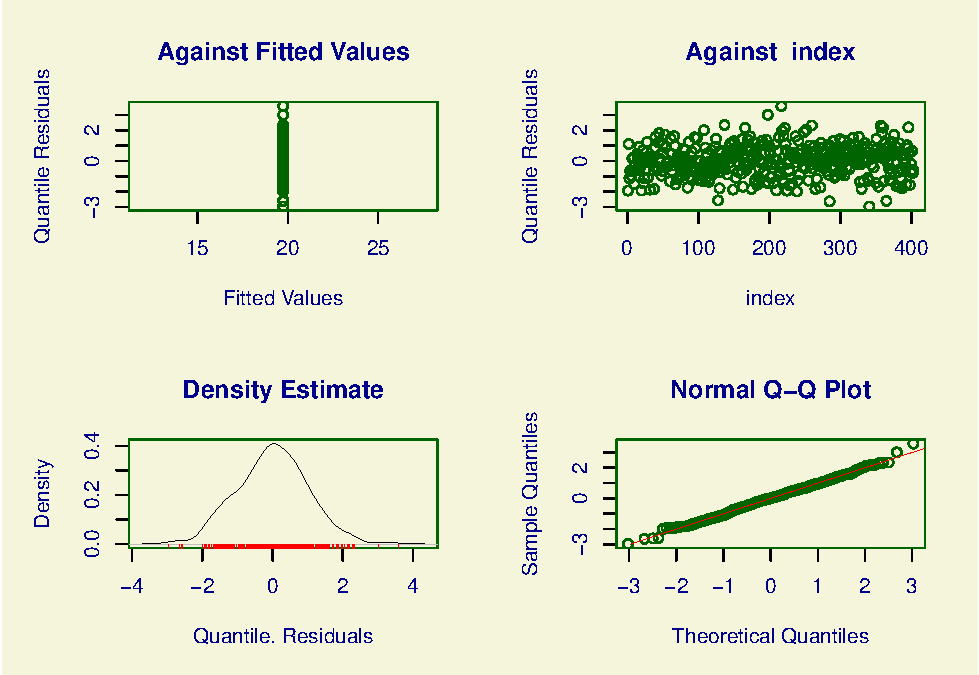
\includegraphics{assignment_q1_bmi_files/figure-latex/unnamed-chunk-8-2.pdf}

\begin{verbatim}
## ******************************************************************
##        Summary of the Quantile Residuals
##                            mean   =  1.028883e-06 
##                        variance   =  1.002488 
##                coef. of skewness  =  0.03768484 
##                coef. of kurtosis  =  3.121755 
## Filliben correlation coefficient  =  0.9983871 
## ******************************************************************
\end{verbatim}

The choice of distribution can be justified by comparing the Akaike
Information Criterion (AIC) values of the fitted models---the model with
the lowest AIC is typically preferred as it suggests a good fit with
relatively lower complexity.

\hypertarget{c-output-the-parameter-estimates-for-your-chosen-model}{%
\subsubsection{(c) Output the parameter estimates for your chosen
model}\label{c-output-the-parameter-estimates-for-your-chosen-model}}

Using the function summary() and interpret the fitted parameters. (You
may refer to the GAMLSS distribution book Rigby et al.~(2019) {[}2{]}
(or to its earlier version which can be found in the GAMLSS web-site
\url{https://www.gamlss.com}) to find what the distribution parameters
represent (i.e.~location, scale, kurtosis etc.).

Finally, for the chosen model, we can output the parameter estimates and
interpret them according to the distribution's characteristics.

\begin{Shaded}
\begin{Highlighting}[]
\CommentTok{\# Output parameter estimates for the chosen model}
\FunctionTok{summary}\NormalTok{(selected\_model)}
\end{Highlighting}
\end{Shaded}

\begin{verbatim}
## *******************************************************************
## Family:  c("JSU", "Johnson SU") 
## 
## Call:  gamlssML(formula = dbbmi_15$bmi, family = "JSU") 
## 
## Fitting method: "nlminb" 
## 
## 
## Coefficient(s):
##             Estimate  Std. Error   t value   Pr(>|t|)    
## eta.mu    19.7442002   0.1102768 179.04212 < 2.22e-16 ***
## eta.sigma  0.7952701   0.0534317  14.88385 < 2.22e-16 ***
## eta.nu     1.6219117   0.6555621   2.47408   0.013358 *  
## eta.tau    0.7379107   0.1869315   3.94749 7.8974e-05 ***
## ---
## Signif. codes:  0 '***' 0.001 '**' 0.01 '*' 0.05 '.' 0.1 ' ' 1
## 
##  Degrees of Freedom for the fit: 4 Residual Deg. of Freedom   399 
## Global Deviance:     1723.71 
##             AIC:     1731.71 
##             SBC:     1747.7
\end{verbatim}

\begin{Shaded}
\begin{Highlighting}[]
\FunctionTok{print}\NormalTok{(fit\_jsu}\SpecialCharTok{$}\NormalTok{mu.coefficients)}
\end{Highlighting}
\end{Shaded}

\begin{verbatim}
## (Intercept) 
##    19.74395
\end{verbatim}

Interpretation of the parameters will depend on the selected
distribution. For example:

\begin{itemize}
\item
  For a Normal distribution (\texttt{NO}), the parameters are the mean
  (\texttt{mu}) and standard deviation (\texttt{sigma}), representing
  the location and scale of the distribution.
\item
  For a Log-Normal distribution (\texttt{LOGNO}), \texttt{mu} and
  \texttt{sigma} represent the mean and standard deviation of the
  variable's logarithm, indicating the distribution's central tendency
  and spread on a log scale.
\item
  For a Gamma distribution (\texttt{GA}), the parameters might include a
  shape and a scale parameter, reflecting the distribution's skewness
  and scale.
\end{itemize}

Refer to the GAMLSS book or documentation for specific interpretations
of the parameters of your chosen distribution. The interpretation will
help in understanding the characteristics of BMI distribution among
Dutch boys aged 10 to 11, such as its central tendency, variability, and
potential skewness.

\begin{Shaded}
\begin{Highlighting}[]
\CommentTok{\# Function to calculate the fitted density}
\NormalTok{density\_fitted }\OtherTok{\textless{}{-}} \ControlFlowTok{function}\NormalTok{(x) \{}
  \FunctionTok{dJSU}\NormalTok{(x, }\AttributeTok{mu=}\NormalTok{fit\_jsu}\SpecialCharTok{$}\NormalTok{mu.coefficients, }\AttributeTok{sigma=}\NormalTok{fit\_jsu}\SpecialCharTok{$}\NormalTok{sigma.coefficients, }\AttributeTok{nu=}\NormalTok{fit\_jsu}\SpecialCharTok{$}\NormalTok{nu.coefficients, }\AttributeTok{tau=}\NormalTok{fit\_jsu}\SpecialCharTok{$}\NormalTok{tau.coefficients)}
\NormalTok{\}}

\CommentTok{\# Histogram with ggplot}
\NormalTok{p }\OtherTok{\textless{}{-}} \FunctionTok{ggplot}\NormalTok{(dbbmi\_15, }\FunctionTok{aes}\NormalTok{(}\AttributeTok{x=}\NormalTok{bmi15)) }\SpecialCharTok{+}
  \FunctionTok{geom\_histogram}\NormalTok{(}\FunctionTok{aes}\NormalTok{(}\AttributeTok{y=}\NormalTok{..density..), }\AttributeTok{binwidth =} \FloatTok{0.5}\NormalTok{, }\AttributeTok{colour=}\StringTok{"black"}\NormalTok{, }\AttributeTok{fill=}\StringTok{"white"}\NormalTok{) }

\CommentTok{\# Add the fitted model curve}
\NormalTok{p }\OtherTok{\textless{}{-}}\NormalTok{ p }\SpecialCharTok{+} \FunctionTok{stat\_function}\NormalTok{(}\AttributeTok{fun=}\NormalTok{density\_fitted, }\AttributeTok{colour=}\StringTok{"red"}\NormalTok{, }\AttributeTok{linewidth=}\DecValTok{1}\NormalTok{)}
\NormalTok{p}
\end{Highlighting}
\end{Shaded}

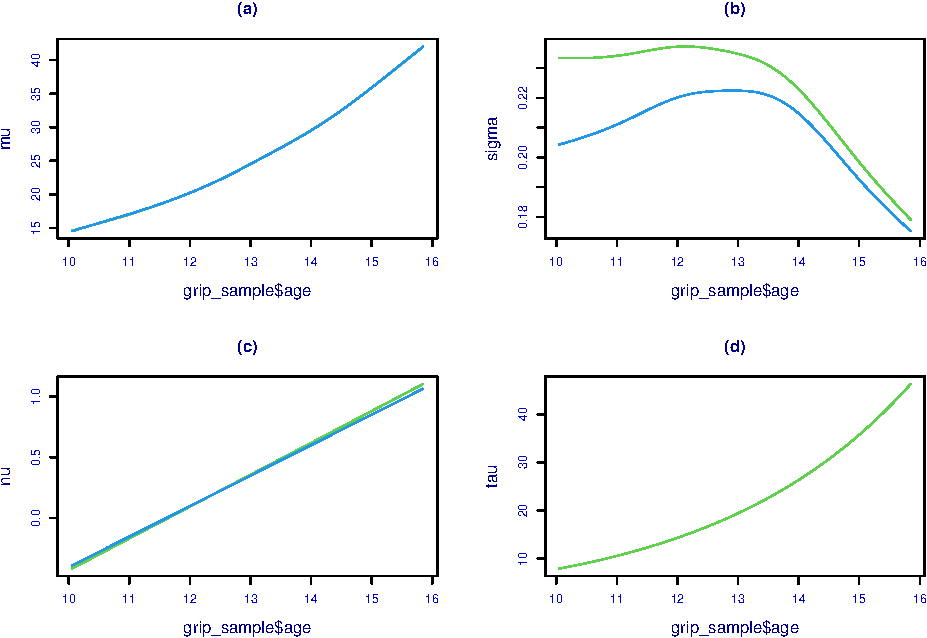
\includegraphics{assignment_q1_bmi_files/figure-latex/unnamed-chunk-10-1.pdf}
